%Version 3 October 2023
% See section 11 of the User Manual for version history
%
%%%%%%%%%%%%%%%%%%%%%%%%%%%%%%%%%%%%%%%%%%%%%%%%%%%%%%%%%%%%%%%%%%%%%%
%%                                                                 %%
%% Please do not use \input{...} to include other tex files.       %%
%% Submit your LaTeX manuscript as one .tex document.              %%
%%                                                                 %%
%% All additional figures and files should be attached             %%
%% separately and not embedded in the \TeX\ document itself.       %%
%%                                                                 %%
%%%%%%%%%%%%%%%%%%%%%%%%%%%%%%%%%%%%%%%%%%%%%%%%%%%%%%%%%%%%%%%%%%%%%

%%\documentclass[referee,sn-basic]{sn-jnl}% referee option is meant for double line spacing

%%=======================================================%%
%% to print line numbers in the margin use lineno option %%
%%=======================================================%%

%%\documentclass[lineno,sn-basic]{sn-jnl}% Basic Springer Nature Reference Style/Chemistry Reference Style

%%======================================================%%
%% to compile with pdflatex/xelatex use pdflatex option %%
%%======================================================%%

%%\documentclass[pdflatex,sn-basic]{sn-jnl}% Basic Springer Nature Reference Style/Chemistry Reference Style


%%Note: the following reference styles support Namedate and Numbered referencing. By default the style follows the most common style. To switch between the options you can add or remove �Numbered� in the optional parenthesis. 
%%The option is available for: sn-basic.bst, sn-vancouver.bst, sn-chicago.bst%  
 
%%\documentclass[sn-nature]{sn-jnl}% Style for submissions to Nature Portfolio journals
%%\documentclass[sn-basic]{sn-jnl}% Basic Springer Nature Reference Style/Chemistry Reference Style
\documentclass[sn-mathphys-num]{sn-jnl}% Math and Physical Sciences Numbered Reference Style 
%%\documentclass[sn-mathphys-ay]{sn-jnl}% Math and Physical Sciences Author Year Reference Style
%%\documentclass[sn-aps]{sn-jnl}% American Physical Society (APS) Reference Style``
%%\documentclass[sn-vancouver,Numbered]{sn-jnl}% Vancouver Reference Style
%%\documentclass[sn-apa]{sn-jnl}% APA Reference Style 
%%\documentclass[sn-chicago]{sn-jnl}% Chicago-based Humanities Reference Style

%%%% Standard Packages
%%<additional latex packages if required can be included here>

\usepackage{graphicx}%
\usepackage{multirow}%
\usepackage{amsmath,amssymb,amsfonts}%
\usepackage{amsthm}%
\usepackage{mathrsfs}%
\usepackage[title]{appendix}%
\usepackage{xcolor}%
\usepackage{textcomp}%
\usepackage{manyfoot}%
\usepackage{booktabs}%
\usepackage{algorithm}%
\usepackage{algorithmicx}%
\usepackage{algpseudocode}%
\usepackage{listings}%
\usepackage{csvsimple}%
%%%%

%%%%%=============================================================================%%%%
%%%%  Remarks: This template is provided to aid authors with the preparation
%%%%  of original research articles intended for submission to journals published 
%%%%  by Springer Nature. The guidance has been prepared in partnership with 
%%%%  production teams to conform to Springer Nature technical requirements. 
%%%%  Editorial and presentation requirements differ among journal portfolios and 
%%%%  research disciplines. You may find sections in this template are irrelevant 
%%%%  to your work and are empowered to omit any such section if allowed by the 
%%%%  journal you intend to submit to. The submission guidelines and policies 
%%%%  of the journal take precedence. A detailed User Manual is available in the 
%%%%  template package for technical guidance.
%%%%%=============================================================================%%%%

%% as per the requirement new theorem styles can be included as shown below
\theoremstyle{thmstyleone}%
\newtheorem{theorem}{Theorem}%  meant for continuous numbers
%%\newtheorem{theorem}{Theorem}[section]% meant for sectionwise numbers
%% optional argument [theorem] produces theorem numbering sequence instead of independent numbers for Proposition
\newtheorem{proposition}[theorem]{Proposition}% 
%%\newtheorem{proposition}{Proposition}% to get separate numbers for theorem and proposition etc.

\theoremstyle{thmstyletwo}%
\newtheorem{example}{Example}%
\newtheorem{remark}{Remark}%

\theoremstyle{thmstylethree}%
\newtheorem{definition}{Definition}%

\raggedbottom
%%\unnumbered% uncomment this for unnumbered level heads

\begin{document}

\title[Article Title]{Overpriced and Undersupplied: Density as a Measure of Demand in Large US Apartment Markets}

%%=============================================================%%
%% GivenName	-> \fnm{Joergen W.}
%% Particle	-> \spfx{van der} -> surname prefix
%% FamilyName	-> \sur{Ploeg}
%% Suffix	-> \sfx{IV}
%% \author*[1,2]{\fnm{Joergen W.} \spfx{van der} \sur{Ploeg} 
%%  \sfx{IV}}\email{iauthor@gmail.com}
%%=============================================================%%

\author*[1,2]{\fnm{First} \sur{Author}}\email{iauthor@gmail.com}

\author[2,3]{\fnm{Second} \sur{Author}}\email{iiauthor@gmail.com}
\equalcont{These authors contributed equally to this work.}

\author[1,2]{\fnm{Third} \sur{Author}}\email{iiiauthor@gmail.com}
\equalcont{These authors contributed equally to this work.}

\affil*[1]{\orgdiv{Department}, \orgname{Organization}, \orgaddress{\street{Street}, \city{City}, \postcode{100190}, \state{State}, \country{Country}}}

\affil[2]{\orgdiv{Department}, \orgname{Organization}, \orgaddress{\street{Street}, \city{City}, \postcode{10587}, \state{State}, \country{Country}}}

\affil[3]{\orgdiv{Department}, \orgname{Organization}, \orgaddress{\street{Street}, \city{City}, \postcode{610101}, \state{State}, \country{Country}}}

%%==================================%%
%% Sample for unstructured abstract %%
%%==================================%%

\abstract{We introduce an empirical measure of multifamily demand, based on density changes, and offer evidence of its segmenting and predictive power. Using this variable, we solve for the intersection of supply and demand curves each year for 20 years in each of the hundred largest MSAs in the United States. Over the 2,000 observations, we classified each sample as over or under-supplied and over-or-under-priced, based on the derived market-clearing rents and quantities, relative to observed rents and quantities. Grouping markets this way was highly predictive of their next-twelve-month rent growth, with the under-under group returning 2\% more annually than the over-over group. With this, we provide a better way to understand consumer housing demand; their indifference curve of space versus price; and the impact of supply shocks.}

%%================================%%
%% Sample for structured abstract %%
%%================================%%

% \abstract{\textbf{Purpose:} The abstract serves both as a general introduction to the topic and as a brief, non-technical summary of the main results and their implications. The abstract must not include subheadings (unless expressly permitted in the journal's Instructions to Authors), equations or citations. As a guide the abstract should not exceed 200 words. Most journals do not set a hard limit however authors are advised to check the author instructions for the journal they are submitting to.
% 
% \textbf{Methods:} The abstract serves both as a general introduction to the topic and as a brief, non-technical summary of the main results and their implications. The abstract must not include subheadings (unless expressly permitted in the journal's Instructions to Authors), equations or citations. As a guide the abstract should not exceed 200 words. Most journals do not set a hard limit however authors are advised to check the author instructions for the journal they are submitting to.
% 
% \textbf{Results:} The abstract serves both as a general introduction to the topic and as a brief, non-technical summary of the main results and their implications. The abstract must not include subheadings (unless expressly permitted in the journal's Instructions to Authors), equations or citations. As a guide the abstract should not exceed 200 words. Most journals do not set a hard limit however authors are advised to check the author instructions for the journal they are submitting to.
% 
% \textbf{Conclusion:} The abstract serves both as a general introduction to the topic and as a brief, non-technical summary of the main results and their implications. The abstract must not include subheadings (unless expressly permitted in the journal's Instructions to Authors), equations or citations. As a guide the abstract should not exceed 200 words. Most journals do not set a hard limit however authors are advised to check the author instructions for the journal they are submitting to.}

\keywords{keyword1, Keyword2, Keyword3, Keyword4}

%%\pacs[JEL Classification]{D8, H51}

%%\pacs[MSC Classification]{35A01, 65L10, 65L12, 65L20, 65L70}

\maketitle

\section{Introduction}\label{sec1}
\abstract{We introduce an empirical measure of multifamily demand, based on density changes, and offer evidence of its segmenting and predictive power. Using this variable, we solve for the intersection of supply and demand curves each year for 20 years in each of the hundred largest MSAs in the United States. Over the 2,000 observations, we classified each sample as over or under-supplied and over-or-under-priced, based on the derived market-clearing rents and quantities, relative to observed rents and quantities. Grouping markets this way was highly predictive of their next-twelve-month rent growth, with the under-under group returning 2\% more annually than the over-over group. With this, we provide a better way to understand consumer housing demand; their indifference curve of space versus price; and the impact of supply shocks.}  


The article investigates density as a measure of demand for multifamily real estate in the United States. For much of its history, the United States did not need to concern itself with density. It was a sparsely populated country, and it trailed the average density of other high-income countries sharply for two hundred years. Gradually, this changed. And in 2003, for the first time, the United States exceeded the density of its high-income peers, with 31.69 people per square mile \cite{ourworldindataPopulationDensity}. By 2023, it was 5\% denser than the high-income nation average, and by the end of the century, it is forecasted to be 30\% denser. Perhaps not coincidentally, this period coincided with a time of sharp rent growth. The CPI of shelter doubled between 2000 and 2024, exceeding the growth in CPI-excluding-shelter by 34\% \cite{stlouisfedConsumerPrice}. It was also during this period when rent growth began to exceed wage growth \cite{feiveson2024rent}. If a growing density comes with an acceleration in relative rent growth, then it is likely from the demand side. And this is supported by the younger generations' growing preferences for renting \cite{fanniemaeConsumersFeeling}. But with the average consumer paying 31\% \cite{censusNearlyHalf} of his or her income to rent, a further increase in demand risks overburdening the renter, unless supply increases to compensate. It seems granted that the country is undersupplied housing. Only the quantity of additional supply needed is uncertain: Fannie Mae counts 4.4 million units in just the top 75 metros \cite{betancourt2022us}. But how can a nation be both systematically undersupplied  with overpriced housing, when simultaneously bemoaning recent rent declines caused by oversupply \cite{mott2024ThisRegion}? This seemingly contradictory sentiment belies a lack of a reliable measure of demand. If there were greater transparency into the quantity and price of units demanded, then both the supply and demand sides of the transactions could find an equilibrium. Developers would build in quantities closer to those demanded; and renters could select locations based on their rent-stability and underwrite rent growth in line with wage growth. Economically, we have transparency into the physical number of units in existence and in development. We also have pricing data, showing the average price per rented square foot. But from the demand side, we are lacking. In this article, we focus on a measure of demand outside of the traditional and self-referential variables of occupancy and absorption. We provide evidence that density--approximated by population over rental units--and its change can be used as an accurate, versatile measure of demand. Using this metric we construct demand curves that intersect naturally with supply curves, for each market in the top 100 markets, for each year from 2010 through 2022. The points of intersection, relative to the observed rents and supplies serve to classify a market as over or undersupplied and over or underpriced. Markets that are overpriced and undersupplied favor the landlord and have high average rent growth; markets that are underpriced and oversupplied favor the renter and have low-to-negative average rent growth. Markets that are neither tend to have moderate rent growth, between that of the other two. 

While most existing research on demand focuses on occupancy levels and absorption \cite{anenberg2024volatility} \cite{pyhrr1999real} \cite{mueller1999real}, those two variables share a limitation. Namely, they are both capped at 100\%. A building cannot be 110\% occupied, nor can renters absorb more units than are produced. This system of measurement prohibits demand from ever exceeding supply. When operating in this system, it has become common to attribute rent growth to supply or demand--not both or their relationship. While research agrees that geographic limitations are associated with increased costs of shelter, there is disagreement as to whether it is caused by the supply side or the demand side. Saiz (2010) argues the supply side, claiming that cities constrained by geographic features have increased shelter prices because of the lack of developable land, leading those cities to require higher wages and amenities to compensate for the expensive housing \cite{saiz2010geographic}. Davidoff (2015) argues the demand side, suggesting that cities with geographic features are more desirable places to live and experience more growth than cities without geographic features \cite{davidoff2015supply}. While research agrees more affordable housing is necessary, it disagrees on which side influences rents more. Pennington claims that an increase in both market rate and affordable housing is necessary to lowering rents, while Molloy et al. contend that increasing housing supply will not have a substantial effect on rents, and considering demand side variables are more important \cite{pennington2021does} \cite{molloy2022housing}. We contest that supply and demand should be viewed relative to one another and relative to equilibrium, but without a consistent and agreed upon measure of demand, then the problem becomes knotty. 

In search of a proper demand variable, some research examines occupancy \cite{gabriel2001rental} \cite{sirmans1991determinants} \cite{mueller1999real} and finds that it impacts rent growth. Other research focuses on absorption rates \cite{murray2022housing} \cite{gabriel2001rental} and finds it to be a strong explanatory variable for rent growth as well. 
We do not disagree. We aim to further the explanatory power of demand side variables by introducing one that is not bounded by 1 from above. We find density to be such a variable. If one had clear visibility into number-of-people per rental unit, then demand and utility curves could be derived. Under the assumptions that consumers prefer more space \cite{molloy2022housing}, then knowing the price at which a renter chose to live alone versus take a room mate would indicate the quantity of units demanded and the price at which those units would be demanded. Prior work has explored density, and while density appears to be a net amenity, part of the rent increase associated with higher density may be attributable to the higher cost of providing space. For some renters, increased density can translate to desirable urban living spaces, surrounded by jobs and amenities while for others, it can result in overcrowding and reduced quality of life. Policy induced densification may involve a net cost to renters and first-time homebuyers \cite{ahlfeldt2019economic} \cite{albouy2015driving}. 
  
But that does not fully address the question. None of the previous studies define density as population divided by rental units, but instead as population divided by area or as units divided by area . Not all parts of a city are residential moreover, not all parts are even habitable, due to geographic or other restrictions. These density metrics are not effective in capturing the level of supply relative to the population in an MSA.  

Our main contribution is to provide evidence of the use of density as a measure of demand. Other work has explored demand from an agglomeration point-of-view, modeling the benefits of agglomeration externalities, and exploring how agglomeration affects rents in urban areas \cite{titman2024city} \cite{liu2018vertical}. And that nods to the cyclical unique nature of real estate--where more density can make a more valuable commodity that can in turn produce more density. A paradigm where a renter is willing to pay more for less space in Manhattan, when she could pay less for more space in Houston. MSA-level density and its year-over-year change reveals a proxy of demand which indicates whether rents will grow in the near-term. We call this metric implied demand and show that it provides evidence of over or undersupply and over or underpricing.  

\begin{figure}[H]
	\centering
	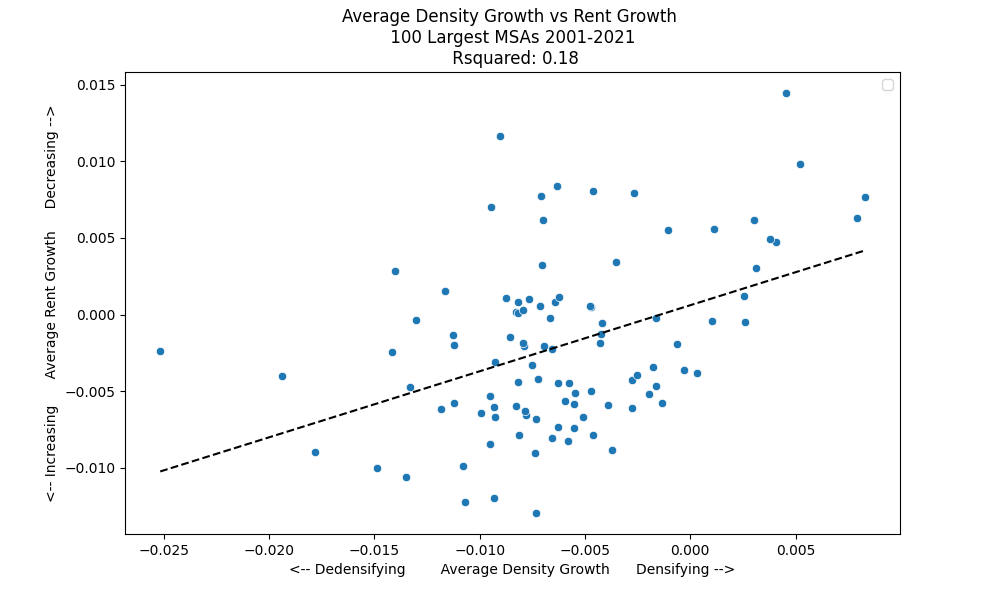
\includegraphics[width=0.9\textwidth]{"C:/Users/mlarriva/Documents/GitHub/demand_density/Figs/density_growth_vs_rent_growth.png"}
	\caption{At the market level, markets that increase in density have higher real rent growth. Markets that decrease in density on average have lower rent growth. We postulate that markets with higher rents force renters to cohabitate i.e., increase the density of people per unit. Alternatively, the renter can move markets for a lower rent at a less dense space.}\label{fig1}
\end{figure}

\begin{figure}[H]
	\centering
	\includegraphics[width=0.9\textwidth]{"C:/Users/mlarriva/Documents/GitHub/demand_density/Figs/national_example.png"}
	\caption{But at the national level, years of increased density are associated with lower rent growth than years of decreased density. This global curve suggests an intuitive demand curve: a renter opts for more space (less density) and is willing to pay more for it; or the renter chooses less space (more density) and is willing to pay less.}\label{fig4}
\end{figure}

Our article also speaks to the broader debate of rent affordability, the need for more housing, and the local differences inherent in such discussions. From the owner/developer standpoint, a more useful measure of demand could dampen real estate development cycles, which often result in unexpectedly depressed rents. From the renter's standpoint, a more useful demand metric can help identify locations where rent is likely to grow, maintain, or decrease, relative to inflation.  

Focusing on a panel of the 100 largest metropolitan statistical areas (MSA), their population, rental unit count, and change in rent, we estimate implied demand of each MSA at each of 10 years from 2013 to 2023. We plot this against rent to derive a demand curve. We then take the observed supply growth of each MSA and plot it against rent to derive a supply curve. The intersection of those two curves is the derived point of supply and rent equilibrium. Comparing a market's actual rent to the market's derived rent suggests over or underpricing. Comparing a market's actual supply growth to the market's derived supply growth provides evidence of over or undersupply. We show that by segmenting markets as over or undersupplied and over or underpriced each year, we can effectively forecast the market's next-year rent growth.  

In the next section we discuss measures of demand before presenting details on our proposed variable. The data section describes and analyzes the density data we used, while the Emperical Analysis section presents evidence and illustrates statistical tests performed to evaluate the validity of the classifications. The final section discusses the results and concludes. 
 
\section{Measures of Demand}
\subsection{Existing Measures of Demand}
\subsection{Density as a Measure of Demand}
Density has a network-affect in real estate that is not common to other real assets. A telephone network would be useless if it had only one customer: whom would she call? But if ten people are on the network, the value of the network increases. So too in cities where agglomeration econonmics take effect. This phenomenon makes it so both the employer and employee are better off when there are many other firms in a short distance. The employee has higher employment security knowing he can shift firms if needed. The employer has a larger workforce available so he can scale up if needed. [find a reference]. Socially, the dense city offers ease of connection and more options of recreation. For these reasons, density, or a lack of space, is a worthwile tradeoff. Economically however it means that a renter will pay more for less space.

This occurs both at the unit level and at the city level. A renter may opt out of a 1000-square-foot unit in a suburb for a 500-square-foot unit in a city. Or, she may opt share a 1000 sqare-foot unit with a roomate. When viewed in aggregate, the population of a city and its total rental units provides a valiable quotient we call \textit{rental density index} or RDI. The RDI can be understood as the theoretical density an MSA would incur to house its entire population in rental units. It is not meant as a goal or to have intuitive readthrough but to serve as a reference point for the utility curve of a city's residents. 
The RDI contains latent information regarding homeownership, cohabitation preferences, and family size. The RDI moves slowly over time and is densely concentrated across MSAs. The mean RDI decreases in sync with the observed decrease in people-per-household in the US [find reference].

\section{Data}
\subsection{Real Rent Growth and Inventory at the largest MSAs}
We limit our analysis to the hundred-largest MSAs in the US. To establish the one hundred largest, we examined multifamily inventory at the end of 2001. The largest market in 2001 (and today) was the New York City MSA, with 1,250,237 units. The smallest was Corpus Christi, TX, with 20,783 units. Inventory data is sourced to Costar. To compute real rent growth at the MSA, we begin with Costar's reported "Market Effective Rent Growth 12 Mo." Costar defines this as the Effective Rent Growth for a rolling 12-month value. We chose effective rent growth rather than asking rent growth in order to correctly account for the effect of concessions and to capture more of the impact of potential vacncies. TWe refer to this as "rent growth" throughout this analysis, but in all cases it is effective rent growth year over year. To convert the rent growth from nominal to real, we use the Consumer Price Index for All Urban Consumers: All Items. Using the annual value, as calculated by the average of the monthly values, we take the year-over-year difference to calculate the growth in CPI. We subtract each year's CPI growth from the respective year of rent growth, at each MSA. Ideally, we would use an MSA-specific inflation figure that excluded rent, for each respective city, but this does not exist. The St. Louis Fed discontinued its MSA-specific inflation figures. And while it offers the CPI of services ex rent of shelter, it does not offer the CPI of all items less rent of shelter. We feel despite these shortcomings, measuring real rent by using rent growth and all-item CPI is approrpiate for the purposes of examinig real rent growth relative to other points in time and relative to other markets. The range of rent growth reflects the impact of natural disasters (-19\% in New Orleans in 2005 followed by 28\% in 2006) to industry bubbles (-14\% San Jose 2002) to COVID relocations (22\% Palm Beach, 2022). 

\subsection{Population, and density}
To calculate our measure of density we divide the occupied inventory by the population. Occupancy rates are sourced to Costar on an annual basis. Inventory figures are gathered as described above. And population figures come from Costar who uses Moody's for its demographic data. We call this quotient the \textit{rental density index} or RDI. The RDI ranges from 7 to 65 and gives the number of people in a market per occupied rental unit. Theoretically, if everyone lived in rental units, it would suggest the household size, but of course, that is not the case. The measure follows the overall trend in the US of decreasing density, and as such it is nonstationary. In 1970, 19\% of all households were nonfamily households. In 2022 that number was 36\%. The trend in average is shown below.

\begin{figure}[H]
	\centering
	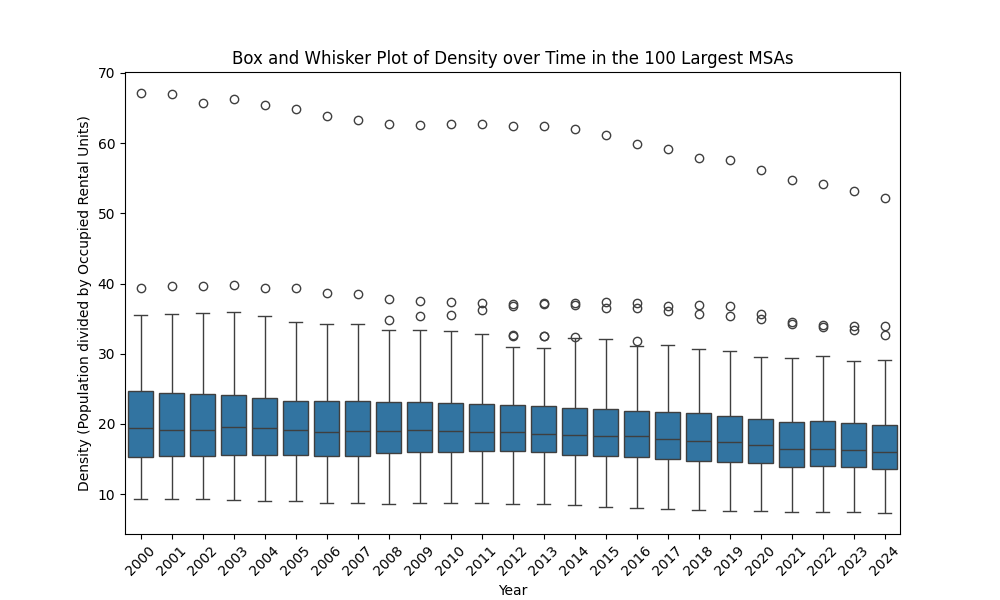
\includegraphics[width=0.9\textwidth]{"C:/Users/datbu/OneDrive/Documents/GitHub/demand_density/Figs/box_whisker_density_time.png"}
	\caption{This is a widefig. This is an example of long caption this is an example of long caption  this is an example of long caption this is an example of long caption}\label{fig1}
\end{figure}

To make the variable stationary and to allow comparisons between markets, and to mute the impact of different rentership percentages by market, we take the year-over-year difference in RDI ($\Delta\text{RDI}$) as our novel demand variable. Descriptive metrics follow
While the RDI indicates preferences across time and region, the change in the rental density index or $\Delta\text{RDI}$ is the focus of this work. The year-over-year change in the RDI is an information-rich variable both alone, in comparison to other MSAs, and in conjunction with rent changes. When combined with the rent per-square-foot the $\Delta\text{RDI}$ indicates when renters would prefer to cohabitate rather than absorb more space. It suggests a level at which more units would be demanded, and it provides insight into the level at which over and undersupply occur. 
Summary metrics follow.

\begin{figure}[H]
	\centering
	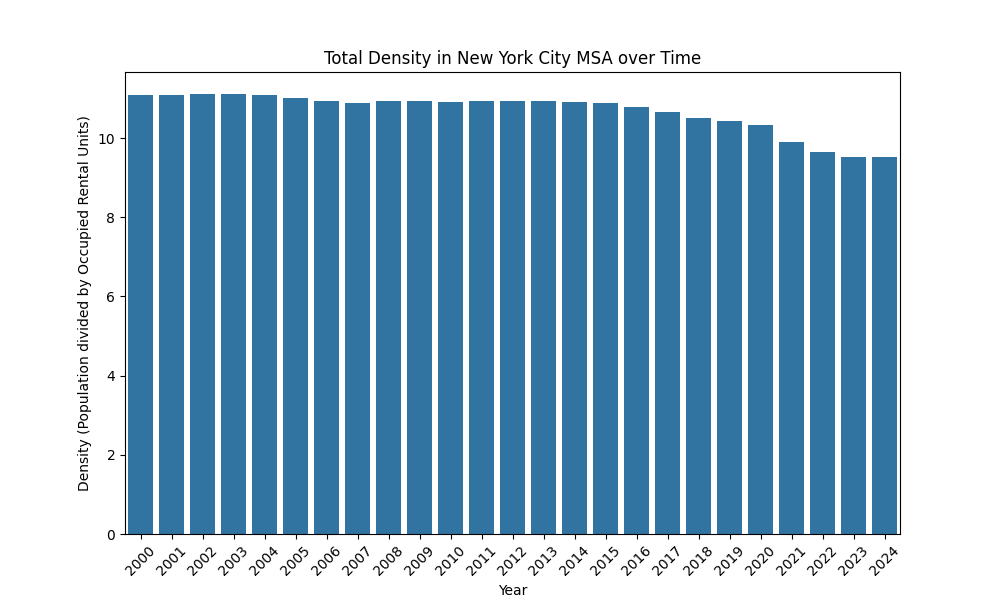
\includegraphics[width=0.9\textwidth]{"C:/Users/datbu/OneDrive/Documents/GitHub/demand_density/Figs/bar_total_density_year.png"}
	\caption{This is a widefig. This is an example of long caption this is an example of long caption  this is an example of long caption this is an example of long caption}\label{fig2}
\end{figure}
\begin{figure}[H]
	\centering
	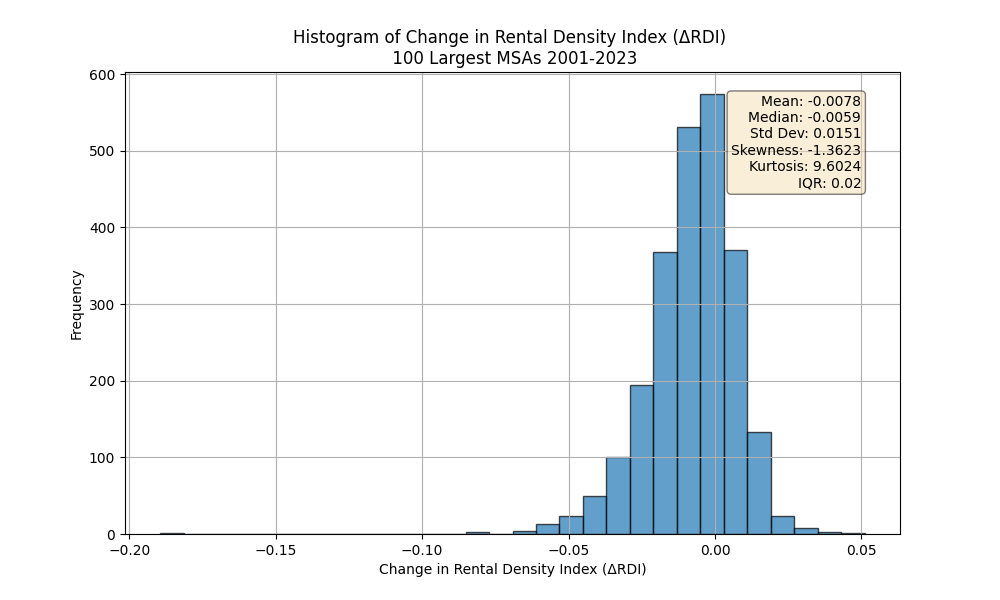
\includegraphics[width=0.9\textwidth]{""C:/Users/datbu/OneDrive/Documents/GitHub/demand_density/Figs/hist_deltardi.png""}
	\caption{This is a widefig. This is an example of long caption this is an example of long caption  this is an example of long caption this is an example of long caption}\label{fig3}
\end{figure}

Nationally, the relationship between $\Delta\text{RDI}$ and rent growth is inverse: rent growth decreases when renters cohabitate; it increases when renters demand their own units and absorb limited stock. This creates a downward sloping demand curve which we can use to find the intersection with the supply curve. 

\begin{figure}[H]
	\centering
	\includegraphics[width=0.9\textwidth]{"C:/Users/datbu/OneDrive/Documents/GitHub/demand_density/Figs/national_example.png"}
	\caption{This is a widefig. This is an example of long caption this is an example of long caption  this is an example of long caption this is an example of long caption}\label{fig4}
\end{figure}
\subsection{Controls}
\subsection{Descriptive Statistics}


\section{Empirical Evidence}\label{sec2}
Our objective is to analyze $\Delta\text{RDI}$ as a meaningful measure of demand. We do so by creating a demand curve for each MSA, for each year, plotting the trailing-10 years of $\Delta\text{RDI}$ against real rent per square foot. We intersect this line with the supply line. The supply line is defined as new supply as a percent of existing stock versus the real rent per square foot. The intersection of the supply and our demand curve produces the derived quantity (q*) and derived price (p*). These derived values (p*,q*) may be higher or lower than the actual market price and supply values (p,q). If the derived price (p*) is greater than (less than) p, then we say a market is underpriced (overpriced). If the derived quantity q* is greater than (less than) the observed quantity q then we say a market is undersupplied (oversupplied).

In any point in time, a market can then be in one of four states: overpriced undersupplied; overpriced oversupplied; underpriced undersupplied; underpriced oversupplied. We can call an overpriced and undersupplied market a landlord-favorable market. Conversely a market that is underpriced and oversupplied would be a renter-favorable market. Other combinations are neither renter nor landlord-favorable. We would expect lanlord-favorable markets to see higher rent growth the following year, as inventory is slow-moving prices will adjust up as landlords see there are few alternatives for new or renewing renters. Conversely, we would expect a renter-favorable market to see lower rent growth the following year, as landlords lower rents to incentivize renters to fill their vacant units. 

\begin{table}[h!]
\centering
\begin{tabular}{cc|c|c|}
\multicolumn{2}{c}{} & \multicolumn{2}{c}{\textbf{Pricing}} \\
\multicolumn{2}{c}{} & \textbf{Overpriced} & \textbf{Underpriced} \\
\cmidrule{3-4}
\multirow{2}{*}{\textbf{Supply}} & \textbf{Oversupplied} & Neutral & Renter Friendly \\\cmidrule{2-4}
 & \textbf{Undersupplied} & Landlord Friendly & Neutral \\
\bottomrule
\end{tabular}
\caption{Hypothesized NTM real rent-growth outcomes based on mispricing and mis-supplying}
\end{table}


\begin{algorithm}
	\caption{Segment Markets Into Over/Underpriced and Over/Undersupplied}\label{alg:market_segmentation}
	\begin{algorithmic}[1]
		\For{each year $y$ from [2010 to 2022]}
		    \For{each market $m$ in the top 100 markets}
		        \State Using the trailing 10 years' data...
		        \State $demandcurve$ = linear regression of  $\Delta\text{RDI}$  vs price-psf
		        \State $supplycurve$ = linear regression of supply growth vs price-psf
		        \State $(q^*, p^*)$ = Intersection of $supplycurve$ and $demandcurve$
		        \State $(q, p)$ = market's actual supply and price-per-square-foot in year $y$
		        \If{$q^* > q$} 
		            \If{$p^* > p$}
		                \State Assign market $m$ in year $y$ to Group \textbf{OversuppliedUnderpriced}
		            \Else
		                \State Assign market $m$ in year $y$ to Group \textbf{OversuppliedOverpriced}
		            \EndIf
		        \Else
		            \If{$p^* > p$}
		                \State Assign market $m$ in year $y$ to Group \textbf{UndersuppliedUnderpriced}
		            \Else
		                \State Assign market $m$ in year $y$ to Group \textbf{UndersuppliedOverpriced}
		            \EndIf
		        \EndIf
		    \EndFor
		\EndFor
	\end{algorithmic}
\end{algorithm}


As an example:


\begin{filecontents*}{}


\section{Emperical Analysis}



Equations in \LaTeX\ can either be inline or on-a-line by itself (``display equations''). For
inline equations use the \verb+$...$+ commands. E.g.: The equation
$H\psi = E \psi$ is written via the command \verb+$H \psi = E \psi$+.

For display equations (with auto generated equation numbers)
one can use the equation or align environments:
\begin{equation}
    \|\tilde{X}(k)\|^2 \leq\frac{\sum\limits_{i=1}^{p}\left\|\tilde{Y}_i(k)\right\|^2+\sum\limits_{j=1}^{q}\left\|\tilde{Z}_j(k)\right\|^2 }{p+q}.\label{eq1}
\end{equation}
where,
\begin{align}
    D_\mu        & =  \partial_\mu - ig \frac{\lambda^a}{2} A^a_\mu \nonumber                            \\
    F^a_{\mu\nu} & = \partial_\mu A^a_\nu - \partial_\nu A^a_\mu + g f^{abc} A^b_\mu A^a_\nu \label{eq2}
\end{align}

\section*{Declarations}

Some journals require declarations to be submitted in a standardised format. Please check the Instructions for Authors of the journal to which you are submitting to see if you need to complete this section. If yes, your manuscript must contain the following sections under the heading `Declarations':

\begin{itemize}
    \item Funding
    \item Conflict of interest/Competing interests (check journal-specific guidelines for which heading to use)
    \item Ethics approval and consent to participate
    \item Consent for publication
    \item Data availability
    \item Materials availability
    \item Code availability
    \item Author contribution
\end{itemize}

\noindent
If any of the sections are not relevant to your manuscript, please include the heading and write `Not applicable' for that section.

%%===================================================%%
%% For presentation purpose, we have included        %%
%% \bigskip command. Please ignore this.             %%
%%===================================================%%
\bigskip
\begin{flushleft}%
    Editorial Policies for:

    \bigskip\noindent
    Springer journals and proceedings: \url{https://www.springer.com/gp/editorial-policies}

    \bigskip\noindent
    Nature Portfolio journals: \url{https://www.nature.com/nature-research/editorial-policies}

    \bigskip\noindent
    \textit{Scientific Reports}: \url{https://www.nature.com/srep/journal-policies/editorial-policies}

    \bigskip\noindent
    BMC journals: \url{https://www.biomedcentral.com/getpublished/editorial-policies}
\end{flushleft}

\begin{appendices}

    \section{Section title of first appendix}\label{secA1}

    An appendix contains supplementary information that is not an essential part of the text itself but which may be helpful in providing a more comprehensive understanding of the research problem or it is information that is too cumbersome to be included in the body of the paper.

    %%=============================================%%
    %% For submissions to Nature Portfolio Journals %%
    %% please use the heading ``Extended Data''.   %%
    %%=============================================%%

    %%=============================================================%%
    %% Sample for another appendix section			       %%
    %%=============================================================%%

    %% \section{Example of another appendix section}\label{secA2}%
    %% Appendices may be used for helpful, supporting or essential material that would otherwise 
    %% clutter, break up or be distracting to the text. Appendices can consist of sections, figures, 
    %% tables and equations etc.

\end{appendices}

%%===========================================================================================%%
%% If you are submitting to one of the Nature Portfolio journals, using the eJP submission   %%
%% system, please include the references within the manuscript file itself. You may do this  %%
%% by copying the reference list from your .bbl file, paste it into the main manuscript .tex %%
%% file, and delete the associated \verb+\bibliography+ commands.                            %%
%%===========================================================================================%%

\bibliography{bib}% common bib file
%% if required, the content of .bbl file can be included here once bbl is generated
%%\input sn-article.bbl


\end{document}
